\documentclass{article} % For LaTeX2e
\usepackage{nips13submit_e,times}
\usepackage{hyperref}
\usepackage{url}
\usepackage{amsmath}
\usepackage{amsfonts}
\usepackage{breakurl}
\usepackage{graphicx}
\usepackage{caption}
\usepackage{subcaption}
\usepackage{float}
\usepackage{fancyvrb}
\usepackage{booktabs}
\usepackage[font=footnotesize,labelfont=bf]{caption}
% \documentstyle[nips13submit_09,times,art10]{article} % For LaTeX 2.09
\bibliographystyle{ieeetr}

\title{Modeling Civil Conflict and Aid Delivery in Uganda}


\author{
Peter J.~Bull \\
Institute for Applied Computational Science\\
Harvard University\\
52 Oxford Street \\
Cambridge, MA 02139 \\
\texttt{bull@fas.harvard.edu} \\
\And
Isaac M.~Slavitt \\
Institute for Applied Computational Science\\
Harvard University\\
52 Oxford Street \\
Cambridge, MA 02139 \\
\texttt{slavitt@fas.harvard.edu} \\
}

% The \author macro works with any number of authors. There are two commands
% used to separate the names and addresses of multiple authors: \And and \AND.
%
% Using \And between authors leaves it to \LaTeX{} to determine where to break
% the lines. Using \AND forces a linebreak at that point. So, if \LaTeX{}
% puts 3 of 4 authors names on the first line, and the last on the second
% line, try using \AND instead of \And before the third author name.

\newcommand{\fix}{\marginpar{FIX}}
\newcommand{\new}{\marginpar{NEW}}

\nipsfinalcopy % Uncomment for camera-ready version

\begin{document}


\maketitle

\begin{abstract}
Using MCMC techniques, we model civil conflict in Uganda and optimize the limited relief aid that can be provided in these scenarios. We describe a method to simulate civil conflict events in space and time given historical data about these events. We also optimize the distribution of limited aid resources to refugees from these crises. Modeling aid delivery as a combination of the traveling salesman problem and the knapsack algorithm --- two NP-hard problems --- we find acceptable solutions using stochaastic metaheuristics.
\end{abstract}

\section*{The Data}

The data comes from ACLED (Armed Conflict Location and Event Data Project), which is a dataset with locations, dates, fatalities, motivation, actors involved, and other information about civil conflicts in Africa. Their collection of data on Uganda covers 1997-2013, and they have a real-time tracker of events reported in 2014.\cite{ACLED} The need for an understanding of these patterns of conflict is clear, as ACLED notes:

\begin{quote}
This dataset codes the dates and locations of all reported political violence events in over 50 developing countries. Political violence includes events that occur within civil wars or periods of instability. Although civil war occurrence is decreasing across African countries, new forms of political violence are becoming more common.
\end{quote}

For Uganda, the dataset contains around 4,500 observations of civil violence. Each observation includes the data, location, an quantified estimate for how precise these measures are, a number of fatalities for the event, and the actors involved. Figure \ref{fig:map-points} shows these conflicts scattered on a political map of Uganda.

\begin{figure}
  \centering
  \begin{subfigure}[b]{0.5\textwidth}
    \centering
    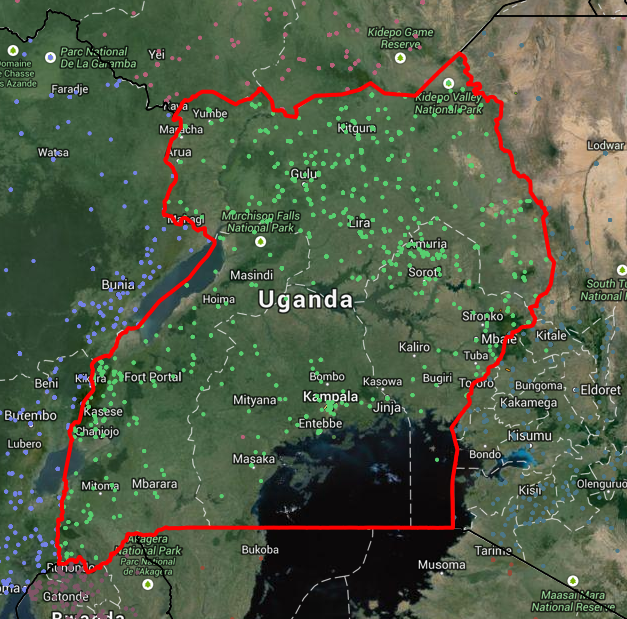
\includegraphics[width=\textwidth]{figures/uganda}
    \caption{Civil conflicts in Uganda 1997-2013.}
    \label{fig:map-points}
  \end{subfigure}~\begin{subfigure}[b]{0.5\textwidth}
    \centering
    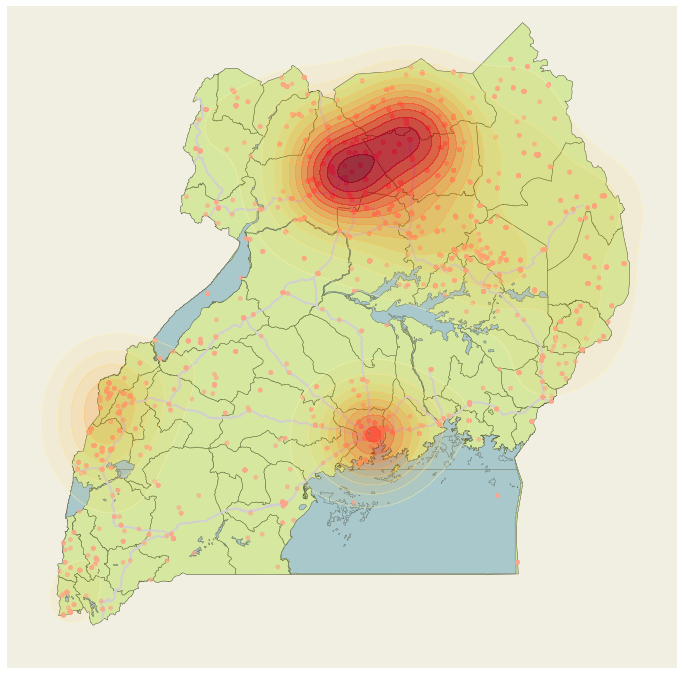
\includegraphics[width=\textwidth]{figures/map-with-smoothed-data}
    \caption{Conflicts with Matérn smoothing.}
    \label{fig:map-smoothed}
  \end{subfigure}
  \caption{Civil conflicts in Uganda.}
  \label{fig:map}
\end{figure}


\section*{Modeling civil conflict events in space}

While we could have trivially fit a Gaussian Process (GP) using the given data, we thought it would be more interesting to apply more directly the MCMC sampling methods learned in this class.  From the MCMC standpoint, it was simple to treat the entire country of Uganda as a probability distribution from which geospatial conflict events could be sampled.  We took historical conflict location data from the entire ACLED data set and smoothed it using a Matérn covariance function.  Figure \ref{fig:map-smoothed} shows this smoothing applied to the same conflicts depicted in \ref{fig:map-points}.

We then discretized that smooth function, which left us with a 2D matrix from which it was easy to sample with any number of samples. Although we experimented with many different methods, we ultimately settled on slice sampling for its favorable, efficient properties. Figure \ref{fig:discretized-matrix} shows this matrix.

\section*{Optimizing Resource Placement and Allocation}

In the second part of this project, we use the first section as both inspiration for the aid delivery analogy and also as a source of randomly sampled data points representing geospatially distributed conflicts.

\subsection*{The Traveling Salesman Problem}

\begin{figure}
	\centering
	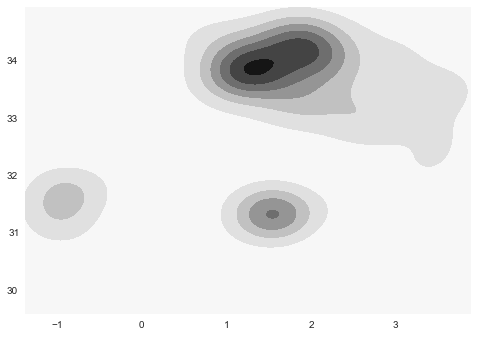
\includegraphics[width=0.6\textwidth]{figures/matern-smoothed-data}
	\caption{Discetized matrix for sampling.}
	\label{fig:discretized-matrix}
\end{figure}

One question of particular interest that we can tackle using techniques from the class is how to route emergency aid
to locations where it is needed.  For concreteness, let's postulate a Red Cross medical or food supply caravan that originates
from the organization's in-country headquarters. This caravan wishes to visit all $n$ emergent locations in order to
deliver needed supplies. They wish to do so in the most efficient manner possible.

This is fundamentally an optimization problem, and one that is well known -- it was first described in 1932 by Karl Menger (shortly after his year here at Harvard as a visiting lecturer) and has been studied extensively ever since.\cite{Menger} Here is the traditional convex optimization specification of the problem:\cite{Winston}


\begin{align*}
\min &\sum_{i=0}^n \sum_{j\ne i,j=0}^nc_{ij}x_{ij} &&  \\
\mathrm{s.t.} & \\
	& x_{ij} \in \{0, 1\} && i,j=0, \cdots, n \\
	& \sum_{i=0,i\ne j}^n x_{ij} = 1 && j=0, \cdots, n \\
	& \sum_{j=0,j\ne i}^n x_{ij} = 1 && i=0, \cdots, n \\
	&u_i-u_j +nx_{ij} \le n-1 && 1 \le i \ne j \le n
\end{align*}

As is clear from the specification, this is an integer linear program (ILP) where:

\begin{itemize}
  \item $x_{ij}$ is a binary decision variable indicating whether we go from location $i$ to location $j$.
  \item $c_{ij}$ is the distance between location $i$ and location $j$.
  \item The objective function is the sum of the distances for routes that we decide to take.
  \item The final constraint ensures that all locations are visited once and only once.
\end{itemize}

\subsection*{Answering complex, realistic questions}

\subsubsection*{Packing the aid truck - adding the Knapsack Problem}

We extend the TSP into a multi-objective optimization problem
where \emph{the contents of the aid trucks} also have an optimization component. Therein lies
the knapsack problem: subject to a volume or weight constraint, and given that different locations
might have very different needs such as food, vaccinations, or emergent medical supplies, \emph{which
supplies do we pack on the trucks}?

Here's the unbounded\footnote{Often, this problem is formulated such that you can only bring one of
each item, but that doesn't make sense here. We want to be able to bring as many types of each type
of aid as we think necessary, and we'll assume that as many as desired are available to load on the
trucks before starting out from HQ.} version of the knapsack problem:

\begin{align*}
\max &\sum_{i=1}^n v_i x_i &&  \\
\mathrm{s.t.} & \\
    & x_i \in \mathbb{Z} \\
    & x_i \geq 0 \\
	& \sum_{i=1}^n w_ix_i \leq W
\end{align*}

In this formulation:

\begin{itemize}
  \item $x_{i}$ is a zero or positive integer decision variable indicating how many units of item $i$
        we load on the truck.
  \item $v_i$ is the utility we get from bringing along item $i$.
  \item $w_i$ is the weight of item $i$.
  \item $W$ is the maximum weight the truck can carry.
\end{itemize}

The problem, of course, is that brute force solution of the TSP is $\mathcal{O}$$(n!)$. Traditional, deterministic
algorithm approaches such as branch-and-bound or branch-and-cut are still impractical for larger numbers of nodes.
In many cases, exhaustive search for global optimality is not even particularly helpful as long as the solution
found is good enough. We will use simulated annealing (SA) to get acceptable solutions to the TSP (c.f. the class lectures
and homework problem).

\begin{figure}
  \centering
  \begin{subfigure}[b]{0.5\textwidth}
    \centering
    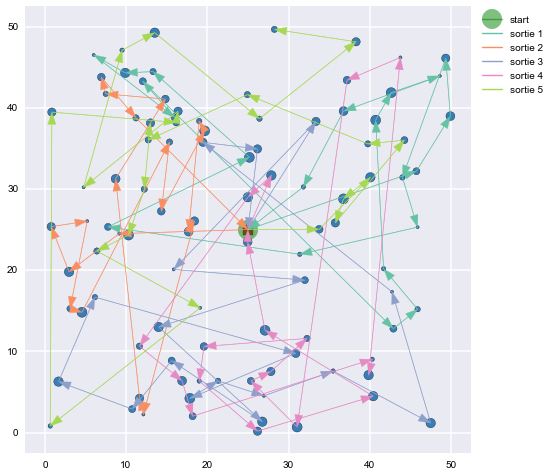
\includegraphics[width=\textwidth]{figures/sorties-5000}
    \caption{After 5,000 iterations.}
  \end{subfigure}~\begin{subfigure}[b]{0.5\textwidth}
    \centering
    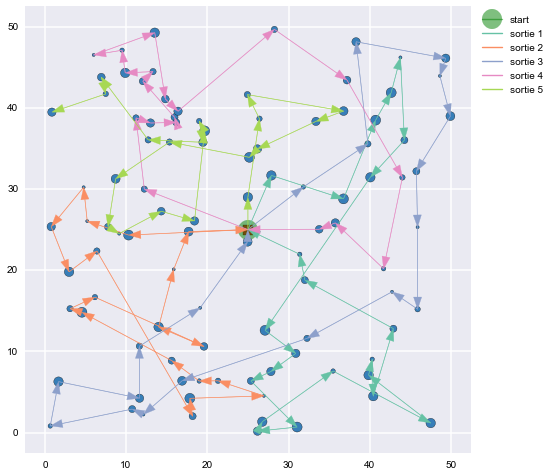
\includegraphics[width=\textwidth]{figures/sorties-20000}
    \caption{After 20,000 iterations.}
  \end{subfigure}
  \begin{subfigure}[b]{\textwidth}
    \centering
    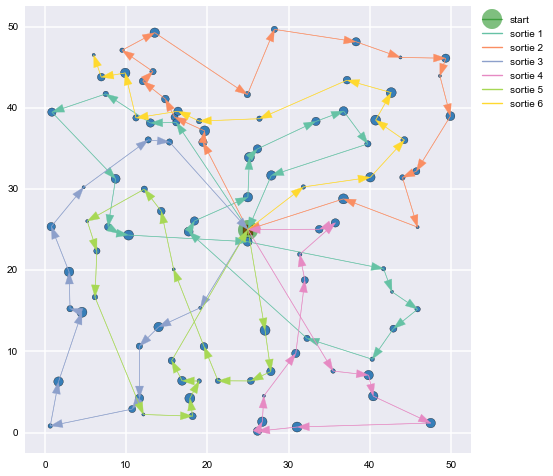
\includegraphics[width=\textwidth]{figures/sorties-100000}
    \caption{After 100,000 iterations.}
  \end{subfigure}
  \caption{Routing for the TSP/Knapsack hybrid.}
  \label{fig:sorties}
\end{figure}

\begin{figure}
	\centering
	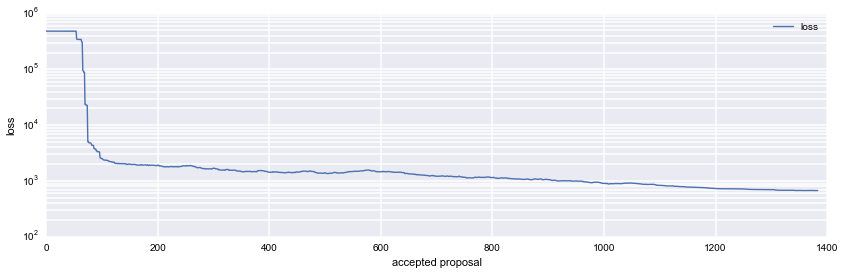
\includegraphics[width=\textwidth]{figures/sorties-loss}
	\caption{Loss function acceptances over 100,000 iterations.}
	\label{fig:sorties-loss}
\end{figure}

\subsubsection*{Finding the optimal site for the resupply location}

Lorem ipsum dolor sit amet, consectetur adipisicing elit, sed do eiusmod tempor incididunt ut labore et dolore magna aliqua. Ut enim ad minim veniam, quis nostrud exercitation ullamco laboris nisi ut aliquip ex ea commodo consequat. Duis aute irure dolor in reprehenderit in voluptate velit esse cillum dolore eu fugiat nulla pariatur. Excepteur sint occaecat cupidatat non proident, sunt in culpa qui officia deserunt mollit anim id est laborum.

\subsubsection*{Factoring in travel time and loss from service delays}

Lorem ipsum dolor sit amet, consectetur adipisicing elit, sed do eiusmod tempor incididunt ut labore et dolore magna aliqua. Ut enim ad minim veniam, quis nostrud exercitation ullamco laboris nisi ut aliquip ex ea commodo consequat. Duis aute irure dolor in reprehenderit in voluptate velit esse cillum dolore eu fugiat nulla pariatur. Excepteur sint occaecat cupidatat non proident, sunt in culpa qui officia deserunt mollit anim id est laborum.

\bibliography{proposal}

\end{document}
